% arara: pdflatex
% !arara: animate: {delay: 80}
% !arara: indent: {overwrite: yes, localSettings: yes}
\documentclass[mathserif]{beamer}
%\documentclass[handout,mathserif]{beamer}
\usepackage{pgfplots}
\usetikzlibrary{positioning}
\usetikzlibrary{fit}
\usetikzlibrary{backgrounds}
\usetikzlibrary{calc}
\usetikzlibrary{shapes}
\usetikzlibrary{mindmap}
\usetikzlibrary{decorations.text}
\pgfplotsset{compat=1.7}

\usetheme{Boadilla}
\usecolortheme{seagull}

% tikzmark command, for shading over items
\newcommand{\tikzmark}[1]{\tikz[overlay,remember picture] \node (#1) {};}

% standard enumeration
\setbeamertemplate{enumerate items}{(\arabic{enumi})}

% default itemize
\setbeamertemplate{itemize items}[circle]

% transparency
\setbeamercovered{transparent=15}

% for resuming lists across frames
\newcounter{savedenum}
\newcommand*{\saveenum}{\setcounter{savedenum}{\theenumi}}
\newcommand*{\resume}{\setcounter{enumi}{\thesavedenum}}

% title
\title{Accessibility in Mathematics}
\subtitle{A collaborative project}
\author[Leavitt, Hughes]{Scot Leavitt \and Chris Hughes}
\institute[PCC]{Portland Community College}
\date{February 19th 2013}
\tikzset{
   invisible/.style={opacity=0},
   visible on/.style={alt=#1{}{invisible}},
   alt/.code args={<#1>#2#3}{%
      \alt<#1>{\pgfkeysalso{#2}}{\pgfkeysalso{#3}} % \pgfkeysalso doesn't change the path
   },
}

%\includeonlyframes{daytoday}

\begin{document}

\begin{frame}
   \maketitle
\end{frame}



\begin{frame}[label=daytoday]{Where do we start?}

   \makebox[\textwidth]{%
      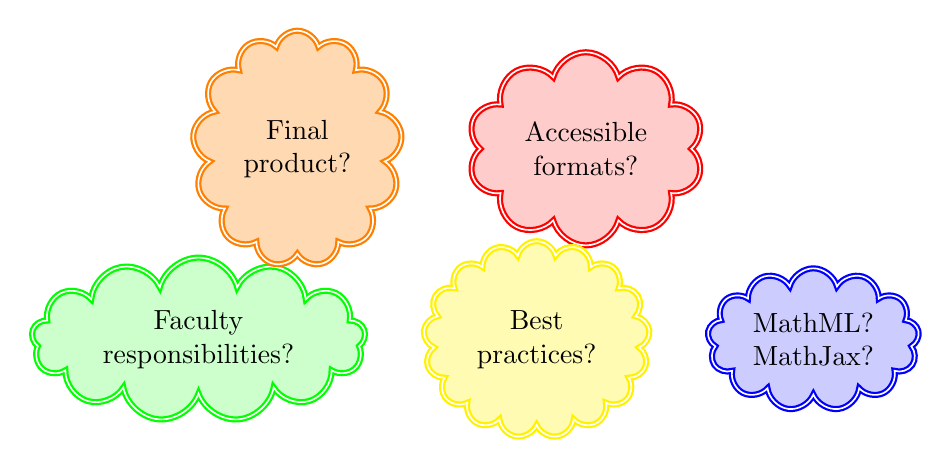
\begin{tikzpicture}[every node/.append style={cloud,draw,thick,align=center}]
         \pause
            \node[draw=red,double,fill=red!20, minimum width=3cm,minimum height=2cm,cloud puffs=10, aspect=1.3](formats){Accessible\\ formats?};
         \pause
            \node[draw=blue,double,cloud,below right=of formats,fill=blue!20, cloud puffs=13, aspect=1.8](mathml)    {MathML?\\MathJax?};
         \pause
            \node[draw=yellow,double,left=0.75cm of mathml, fill=yellow!30, minimum height=2.5cm, cloud puffs=17, aspect=2](final){Best \\ practices?};
         \pause
            \node[draw=green,double,left=0.75cm of final, fill=green!20, cloud puffs=13, aspect=3](best){Faculty\\ responsibilities?};
         \pause
            \node[draw=orange,double,left=of formats, fill=orange!30, minimum width=2cm,minimum height=3cm,cloud puffs=13, aspect=0.9]{Final \\ product?};
      \end{tikzpicture}
   }

\end{frame}

\begin{frame}{Input from department}

   \begin{columns}
      \begin{column}[t]{.65\textwidth}
         What tools do faculty use?

         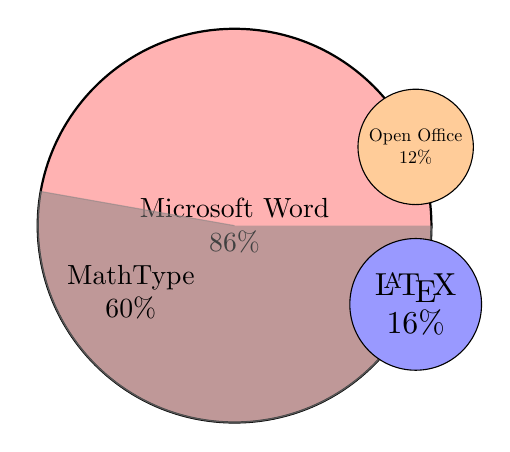
\begin{tikzpicture}[every node/.append style={align=center}]
            \begin{pgfonlayer}{background}
               \node[circle,fill=red!30,draw=black,thick,minimum size=5cm](0,0){Microsoft Word\\ 86\%};
            \end{pgfonlayer}{background}
            \pause
               \visible<2->{\filldraw[gray,opacity=0.5] (2.5,0) arc (0:-190:2.5cm) -- (0,0)node[black,opacity=1,anchor=north east,scale=1,inner sep=.5cm] {MathType \\ 60\%};}
            \pause
               \visible<3->{\node[circle,fill=blue!40,draw=black,scale=1.15] at (2.3,-1){\LaTeX\\16\%};}
            \pause
               \visible<4->{\node[circle,fill=orange!40,draw=black,scale=0.65] at (2.3,1){Open Office\\12\%};}
         \end{tikzpicture}
      \end{column}%
      \pause
         \begin{column}[t]{.35\textwidth}
            Other tools
            \begin{itemize}
               \item Graph
               \item Winplot
               \item GeoGebra
               \item Maple
               \item Excel
               \item PowerPoint
               \item Applets/videos, etc
            \end{itemize}

         \end{column}%
   \end{columns}
\end{frame}


\begin{frame}{Rule of four}

   \centering
   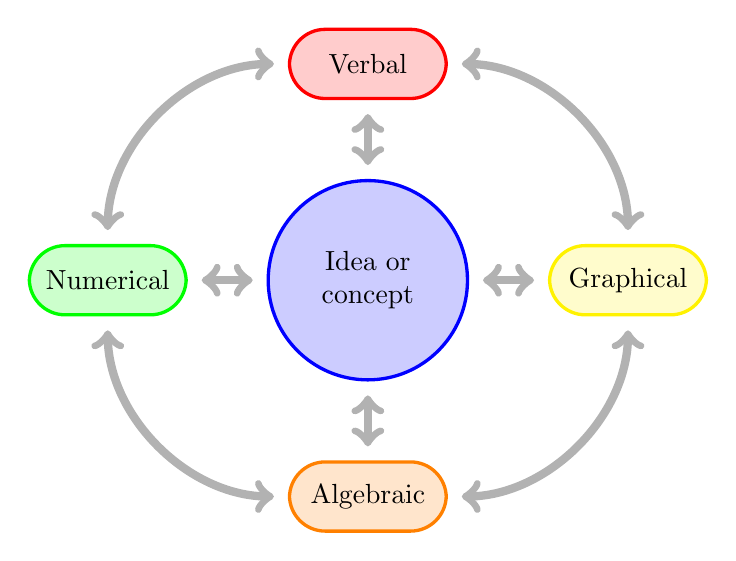
\begin{tikzpicture}[approach/.style={draw,very thick, fill=blue!20, text width=5em,
            text centered, minimum height=2.5em,rounded corners=3ex},
         idea/.style={draw, very thick,fill=blue!40, circle,text width=6em,
            text centered, minimum height=2.5em},
         connections/.style={<->,draw=black!30,line width=3pt,shorten <=5pt,shorten >=5pt},
      ]

      % Draw diagram elements
      \node (idea) [idea,draw=blue,fill=blue!20]  {Idea or concept};
      \pause
         \node (verbal) [approach,draw=red,fill=red!20,above=of idea]  {Verbal};
         \node (tabular) [approach,draw=green,fill=green!20,left=of idea]  {Numerical};
         \node (graphical)[approach,draw=yellow,fill=yellow!20,right=of idea] {Graphical};
         \node (formular)[approach,draw=orange,fill=orange!20,below=of idea] {Algebraic};

         % Draw arrows between elements
         \draw[connections] (idea) -- (formular) ;
         \draw[connections] (idea) -- (verbal);
         \draw[connections] (idea) -- (graphical);
         \draw[connections] (idea) -- (tabular);
         \draw[connections] (verbal.west) to[out=180,in=90](tabular.north) ;
         \draw[connections] (verbal.east) to[out=0,in=90](graphical.north) ;
         \draw[connections] (tabular.south) to[out=-90,in=180](formular.west) ;
         \draw[connections] (graphical.south)to[out=-90,in=0](formular.east);
   \end{tikzpicture}

\end{frame}

\begin{frame}[label=workflow]{Workflow}

   \makebox[\textwidth][c]{%
      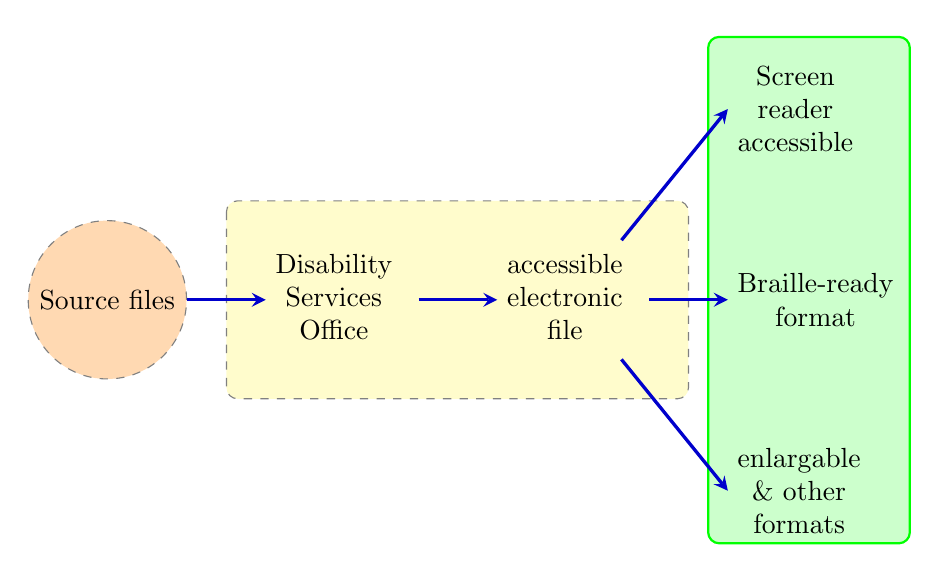
\begin{tikzpicture}[
            outpt/.style={->,blue!80!black,very thick},
            >=stealth,
         every node/.append style={align=center}]
         \node (kaela) at (0,0) {\begin{tabular}{@{}c}Disability\\ Services \\ Office \end{tabular}};
         \pause
            \node (accessfile) [right=of kaela] {\begin{tabular}{@{}c}accessible\\ electronic \\ file \end{tabular}};
            \draw[outpt](kaela)--(accessfile);
            % Draw background
            \begin{pgfonlayer}{background}
               % Left-top corner of the background rectangle
               \path (kaela.west |- kaela.north)+(-0.5,0.5) node (a) {};
               % Right-bottom corner of the background rectanle
               \path (accessfile.east |- accessfile.south)+(+0.5,-0.5) node (c) {};
               % Draw the background
               \path[fill=yellow!20,rounded corners, draw=black!50, dashed]
               (a) rectangle (c);
            \end{pgfonlayer}
         \pause
            \node (screen)[above right=of accessfile]{Screen\\ reader\\ accessible};
            \node (braille)[right =of accessfile]{Braille-ready\\ format};
            \node (enlarge)[below right=of accessfile]{enlargable\\ \& other \\ formats};
            \draw[outpt](accessfile)--(screen.west);
            \draw[outpt](accessfile)--(braille);
            \draw[outpt](accessfile)--(enlarge.west);
            \begin{pgfonlayer}{background}
               % Left-top corner of the background rectangle
               \path (screen.west |- screen.north)+(-0.25,0.25) node (a) {};
               % Right-bottom corner of the background rectanle
               \path (enlarge.east |- enlarge.south)+(0.5,0) node (c) {};
               % Draw the background
               \path[fill=green!20,rounded corners, draw=green,thick]
               (a) rectangle (c);
            \end{pgfonlayer}
         \pause
            \node (source) [left=of kaela,draw=black!50,dashed,circle,fill=orange!30]{Source files};
            \draw[outpt](source)--(kaela);
      \end{tikzpicture}
   }
\end{frame}

\begin{frame}{Stand alone concept}

   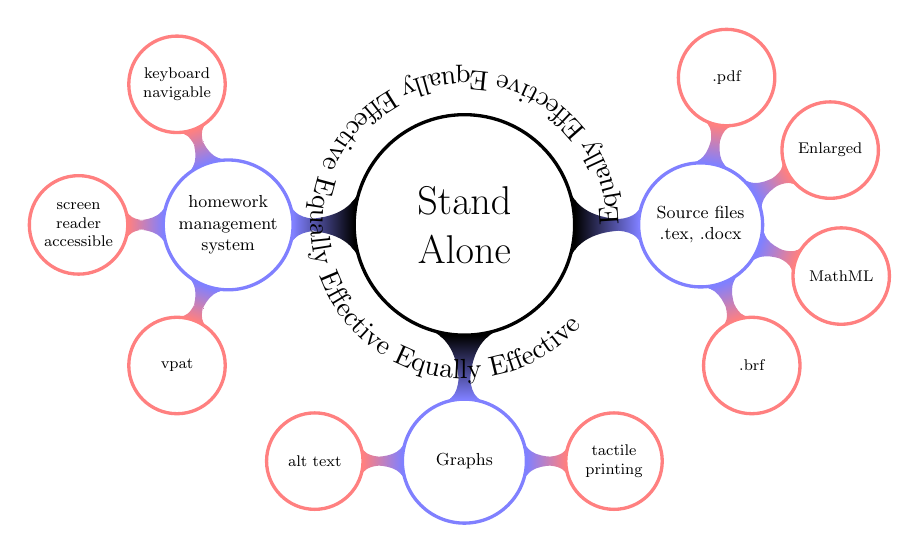
\begin{tikzpicture}[mindmap,
         concept/.append style={fill={none}},
         root concept/.style={concept color=blue},
         level 1 concept/.append style=
         {every child/.style={concept color=blue!50},level distance = 30mm},
         level 2 concept/.append style=
         {every child/.style={concept color=red!50},level distance = 19mm},
         every node/.append style={align=center,scale=0.7},
      ]
      \node [concept,font=\huge] {Stand\\ Alone}
      child[grow=0, visible on=<2->] {node[concept] {Source files .tex, .docx}
         child[grow=80, visible on=<2->]{node[concept] {.pdf}}
         child[grow=30, visible on=<2->]{node[concept] {Enlarged}}
         child[grow=-20, visible on=<2->]{node[concept] {MathML}}
         child[grow=-70, visible on=<2->]{node[concept] {.brf}}
      }
      child[grow=-90,visible on=<3->] {node[concept] {Graphs}
         child[grow=0,visible on=<3->]{node[concept] {tactile printing}}
         child[grow=180,visible on=<3->]{node[concept] {alt text}}
      }
      child[grow=180,visible on=<4->] {node[concept] {homework management system}
         child[grow=110,visible on=<4-> ] {node[concept] {keyboard navigable}}
         child[grow=180,visible on=<4->] {node[concept] {screen reader accessible}}
         child[grow=250,visible on=<4->] {node[concept] {vpat}}
      };
      \node at (0,0) [inner sep=9mm,decorate,circle,decoration=
      {text along path,text={Equally Effective Equally Effective Equally Effective  Equally Effective }}] {};
      %\draw decorate[decoration={text along path,text={Equally Effective}}]
      %{(-3,0) arc (135:45:.5cm)};

   \end{tikzpicture}
\end{frame}

\begin{frame}[c]{What stands alone?}
   % Which content creation tools stand alone?
   \pause
   \begin{columns}
      \begin{column}[c]{.33\textwidth}
         \tikz \node[fill=green!20,draw=green, rounded corners,very thick,inner sep=0mm]{%
            \vbox{%
               \begin{itemize}
                  \item MS Word with MathType
                  \item \LaTeX
                  \item LibreOffice
                  \item Scientific Notebook
                  \item Graphs
                  \item Prepared lecture notes
                  \item Desire2Learn
                  \item WeBWorK
                  \item Videos
               \end{itemize}
            }%
         };
      \end{column}%
      \pause
         \begin{column}[c]{.33\textwidth}
            \tikz \node[fill=orange!20,draw=orange, rounded corners,very thick,inner sep=0mm]{%
               \vbox{%
                  \begin{itemize}
                     \item[] MyMathLab
                  \end{itemize}
               }
            };
            \vfill
         \end{column}%
      \pause
         \begin{column}[c]{.33\textwidth}
            \tikz \node[fill=red!20,
               draw=red,
               rounded corners,
               very thick,
               inner sep=0mm,
               %decorate,decoration={zigzag,segment length=10mm,amplitude=2.0mm},
            ]{%
               \vbox{%
                  \begin{itemize}
                     \item MS Word OMML
                     \item PowerPoint
                     \item TestGen
                     \item GeoGebra applets
                     \item Flash-based applets
                     \item Other media
                  \end{itemize}
               }
            };
         \end{column}
   \end{columns}

\end{frame}


\begin{frame}[fragile]{Collaboration is key}
   \makebox[\textwidth][c]{%
      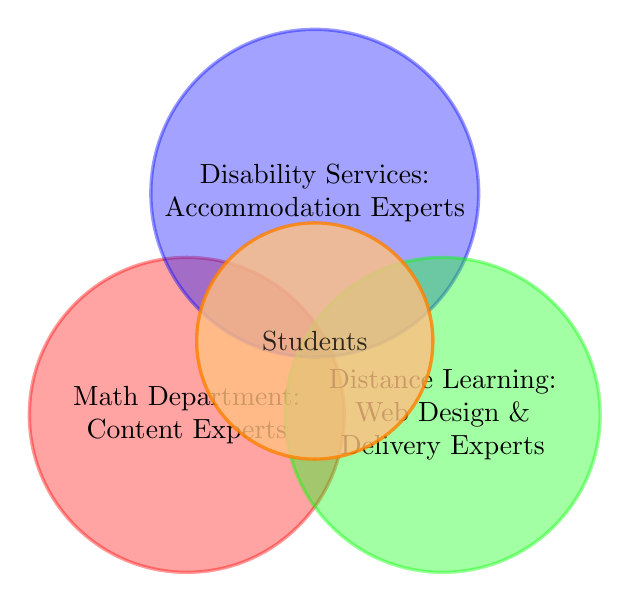
\begin{tikzpicture}[venn circle/.style={draw=#1,
               circle,
               very thick,
               minimum width=4cm,
               text=black,
               fill=#1!90,
               opacity=0.4,
               text opacity=1},
         every node/.append style={align=center}]
         \node [venn circle = red] (A) at (0,0) {Math Department:\\ Content Experts};
         \visible<2->{\node [venn circle = blue] (B) at (60:3.25cm) {Disability Services:\\ Accommodation Experts};}
         \visible<3->{\node [venn circle = green] (C) at (0:3.25cm) {Distance Learning:\\ Web Design \&\\Delivery Experts};}
         \visible<4->{\node[circle,fill=orange!50,draw=orange,very thick,opacity=0.8,minimum width=3cm] at (barycentric cs:A=1/3,B=1/3,C=1/3 ){Students};}
      \end{tikzpicture}
   }
\end{frame}

\end{document}
